\documentclass[
  paper=a4,
  parskip=half,
  fontsize=12pt,
  listof=toc,
  titlepage,
  headsepline,
  footsepline,
]{scrartcl}

% enable UTF-8 text input
\usepackage[utf8]{inputenc}

% DOCUMENT METADATA

\author{Guybrush Threepwood}
\title{Seasonality of Leather Jacket Demand}
\subject{Market Report}

% PREAMBLE

%!TeX root = ../index.tex

% BASICS

% make 3rd party packages behave well with scrartcl
\usepackage{scrhack}

% simple arithmetics
\usepackage{calc}

% language support
\usepackage[american]{babel}

% advanced support for quotations
\usepackage[
  autostyle % adapt quote style to document language
]{csquotes}

% color support
\usepackage[dvipsnames,table,hyperref,fixinclude]{xcolor}

% graphics support
\usepackage[]{graphicx}

% extend file name support for graphicx package
\usepackage[
  extendedchars,
  encoding,
  multidot,
  space,
  filenameencoding=utf8,
]{grffile}

% hyperlink support
\usepackage[
  breaklinks,
  pdfusetitle
]{hyperref}

% bibliography support
\usepackage[
  backend=biber,
  style=authoryear,
  labeldate=year,
  sortcites=true,
  sorting=nyt,
  block=space,
  maxnames=2,
  minnames=1,
  dashed=false
]{biblatex}

% glossaries and acronyms
\usepackage[
    acronym,
    toc=true,
]{glossaries}

% FORMATTING

% micro-typography support (makes most fonts look a little nicer)
\usepackage{microtype}

% support for controlling line spacing
\usepackage{setspace}

% format captions
\usepackage[font=small,labelfont=bf]{caption}

% easily control widow and club penalties
\usepackage[
  defaultlines=4, % keep at least x lines before/after a page break
  all, % apply to whole document
]{nowidow}

% customize list environments
\usepackage{enumitem}

% support for code listings
\usepackage{minted}

% wrapt text around figures
\usepackage{wrapfig}

% MISC

% useful blindtext in document language
\usepackage{blindtext}

% support for placing todo notes in margins
\usepackage[obeyFinal,color=Red,textsize=tiny]{todonotes}


%!TeX root = ../../index.tex

\usepackage[
  %showframe, % draw the layout frame for "debugging"
  top=3cm,
  bottom=2cm,
  left=3.5cm,           % 3.5 + 0.5 Bindingoffset
  right=3cm,
  bindingoffset=0.5cm,
  headheight=22pt,
  headsep=1.25cm-\headheight, % pagetop to header = 1.25cm
  % footheight=\baselineskip,
  footskip=0.75cm, % pagebottom to footer = 1.25cm
  marginparsep=0.3cm,
  marginpar=3.5cm-\marginparsep,
]{geometry}

\setlength{\footheight}{22pt}

%!TeX root=../../index.tex

% include chapter/section titles in headers
\usepackage[
    automark,
]{scrlayer-scrpage}


% Header
\chead[]{}
\ihead[]{}
\ohead[]{\rightmark}

% Footer
\cfoot[]{}
\ifoot[]{}
\ofoot[\pagemark]{\pagemark}

%!TeX root=../../index.tex

%  make \paragraph and \subparagraph behave like small headings
\RedeclareSectionCommands[
    beforeskip=-1sp,
    afterskip=1sp,
    %indent=0pt
]{paragraph,subparagraph}

% Use numbers also for level 1 nested enumerations
\renewcommand{\labelenumii}{\theenumii}
\renewcommand{\theenumii}{\theenumi.\arabic{enumii}.}

%!TeX root = ../index.tex

% support modern fonts
\usepackage[T1]{fontenc}

% sans font that looks similar to Arial
\usepackage{helvet}

% serif font that looks similar to Times New Roman
\usepackage{mathptmx}

% !TeX root = ../../index.tex

\setminted{
  baselinestretch=1.2,
  fontsize=\footnotesize,
  breaklines,
  frame=lines,
  framesep=2mm,
  tabsize=2,
  autogobble
}


% setup hyperref after all packages have been loaded
\hypersetup{
  colorlinks=true,
  allcolors=black,
}

% setup acronyms
% !TeX root = ../index.tex

% \newacronym{cpu}{CPU}{Central Processing Unit}
% \glsunset{cpu}


\makenoidxglossaries{}

% setup bibliography
\addbibresource{assets/bibliography.bib}

% set base path for graphics
\graphicspath{{assets/img}}

% DOCUMENT

\begin{document}

% FRONTMATTER

\maketitle

\clearpage

% use roman page numerals to number frontmatter pages
\pagenumbering{Roman}

% use plain headers
\pagestyle{plain.scrheadings}

% start numbering pages at 2, to include cover page
\setcounter{page}{2}

% use single line spacing to make lists more compact
\singlespacing

\tableofcontents

\clearpage

\listoffigures

\clearpage

% use to change the title of the list of listings
% \renewcommand{\listoflistingscaption}{Quellcodeverzeichnis}
\listoflistings

\clearpage

\setlist[description]{leftmargin=!, labelwidth=4em}

\printnoidxglossary[
    type=\acronymtype,
    sort=nocase,
    nogroupskip,
    nopostdot,
    nonumberlist
]

\setlist[description]{style=standard}

\newcounter{frontpagecount}
\addtocounter{frontpagecount}{\value{page}}

\clearpage

% CONTENT

% use arabic numerals for numbering content pages
\pagenumbering{arabic}

% use the default header style
\pagestyle{scrheadings}

% count content pages from 1
\setcounter{page}{1}

% MS Word does line spacing wrong.
% To get true one-half spacing use '\onehalfspacing'.
% To get something similar to MS Word, use '\setstretch{1.5}'.
\setstretch{1.5}

% !TeX root = ../index.tex

\section{Overview}

The paper \citetitle{mcsherry_privacy_2009} by \citeauthor{mcsherry_privacy_2009} presents the design and implementation of a framework for privacy-preserving data analysis---\gls[]{pinq}.
Their design provides an SQL-like query language and leverages differential privacy to provide formal guarantees towards the \emph{degree} of privacy that a certain query provides.
\gls[]{pinq} is implemented as a wrapper around \gls[]{linq}---a declarative, SQL-like query language integrated into the C\# programming language.
\parencite[][]{mcsherry_privacy_2009}

\section{Context}

The paper can be considered a seminal work in the field of differential privacy with Google Scholar showing 1550 other works that reference it.\footnote{\href{https://scholar.google.com/scholar?q=mcsherry+privacy+integrated+queries}{scholar.google.com}}
It is referenced in multiple surveys in the field of differential privacy \parencites{dwork_differential_2008}{hassan_differential_2019}{xiao_edge_2019}, as well as in a book on the mathematical basis of differential privacy \parencite[]{dwork_algorithmic_2014}.
While the paper itself heavily leans on the two foundational papers for differential privacy \cite[]{dwork_calibrating_2006} and \cite[]{dwork_differential_2006}, its other references mostly serve to differentiate from other works in the field.

\section{Differential Privacy}

Differential privacy forms the theoretical foundation for \gls[]{pinq}.
It is a new way of thinking about privacy that was first articulated by \cite[]{dwork_differential_2006}.

The idea behind differential privacy is that, instead of providing absolute guarantees about whether information leakage will occur or not, mechanisms may provide the relative guarantee that information leakage is just as likely to occur whether a certain record is present in the data set or not.
Thereby, differential privacy guarantees an individual that they gain only very little by not participating in a data set with their data. \parencite[]{dwork_differential_2006}

A mechanism fulfills the requirement of differential privacy if it produces very similar outputs for any two data sets A and B if the two data sets are very similar to each other \cite[]{dwork_differential_2006}.
In other words, the inclusion of a single or a small number of records in a data set has no significant impact on the output of a mechanism that fulfills this requirement.
Therefore, it makes very little difference whether an individual's data is included within a data set, as long as that individuals's data only makes up a small portion of the overall set.

Such mechanisms feature the parameter $\epsilon$ which can be thought of the degree to which the mechanism leaks information.
It may also be regarded as the privacy-\enquote{cost} of an operation. 
High values for $\epsilon$ generally result in more accurate results but also in more information leakage.
\parencite[]{dwork_differential_2006}

\cite[]{mcsherry_privacy_2009} outlines multiple aggregation differentially-private aggregation mechanisms.
The simplest of which is the noisy count, which releases the number of records in a data set but adds symmetric exponential noise to the result.
The intensity of the noise is controlled via $\epsilon$, with higher values meaning less noise.
Next to \texttt{NoisyCount} their implementation also includes among others \texttt{NoisySum}, \texttt{NoisyAvg}, and \texttt{NoisyMed}.

In addition to the aggregation mechanisms, the paper introduces a range of transformation operations that have a stable (i.e. constant) impact on the privacy implication of a query.
The transformations offered by \gls[]{pinq} include among others \texttt{Where}, \texttt{Select}, \texttt{GroupBy} and \texttt{Join}.
For example, \texttt{Where} has a stability of one since the presence (or absence) of a single input record has an impact of at most one output record.
The traditional notion of the \texttt{Join} as a cartesian product of the input records however, would mean unbounded stability.
The \gls[]{pinq} implementation of the \texttt{Join} operation therefore first groups the two input data sets by the join keys and then pairs off the groups with identical keys.
Through this restriction the \gls[]{pinq} \texttt{Join} has a stability of two.
\parencite[]{mcsherry_privacy_2009}

\section{Implementation}

\gls[]{pinq} implements these operations by wrapping the \gls[]{linq} query language which is integrated into the C\# programming language.
\gls[]{linq} provides the \texttt{IQueryable<T>} type which offers operations such as \texttt{Where}, \texttt{Select}, \texttt{GroupBy}, et cetera.
\gls[]{pinq} provides a new type \texttt{PINQueryable<T>} that offers differentially-private operations.
The execution of these operations is not implemented by \gls[]{pinq} instead it wraps around \texttt{IQueryable<T>} and renders every operation to a \gls[]{linq} query while ensuring the necessary operations to conform to the requirements of differential privacy.
Deferring the execution to \gls[]{linq} makes \gls[]{pinq} pretty lightweight---coming in at under 1000 lines of code.
\parencite{mcsherry_privacy_2009}

\texttt{PINQueryable} instances consist of an \texttt{IQueryable} and a \texttt{PINQAgent}.
The latter is a new data type also introduced by the framework.
Aggregations performed via \texttt{PINQueryable} produce a usable result (such as a sum or count) but first test the \texttt{PINQAgent} for whether they may perform the operation by passing it the $\epsilon$ value of the operation.
Transformations produce a new \texttt{PINQueryable} instance with a transformed \texttt{IQueryable} and a new \texttt{PINQAgent}.
These new \texttt{PINQAgent} instances retain a reference to the agent of their origin \texttt{IQueryable} and if queried for whether they permit an operation, they multiply the operation's epsilon with the stability of the appropriate transformation and forward the request with the new $\epsilon$ value to the origin's agent.
Thereby, \gls[]{pinq} enforces propagation of the \enquote{cost} of a query as well as of the responsibility for permitting it back to the original data source(s).
\parencite[]{mcsherry_privacy_2009}

\begin{wrapfigure}{l}{0.6\textwidth}
  \centering
  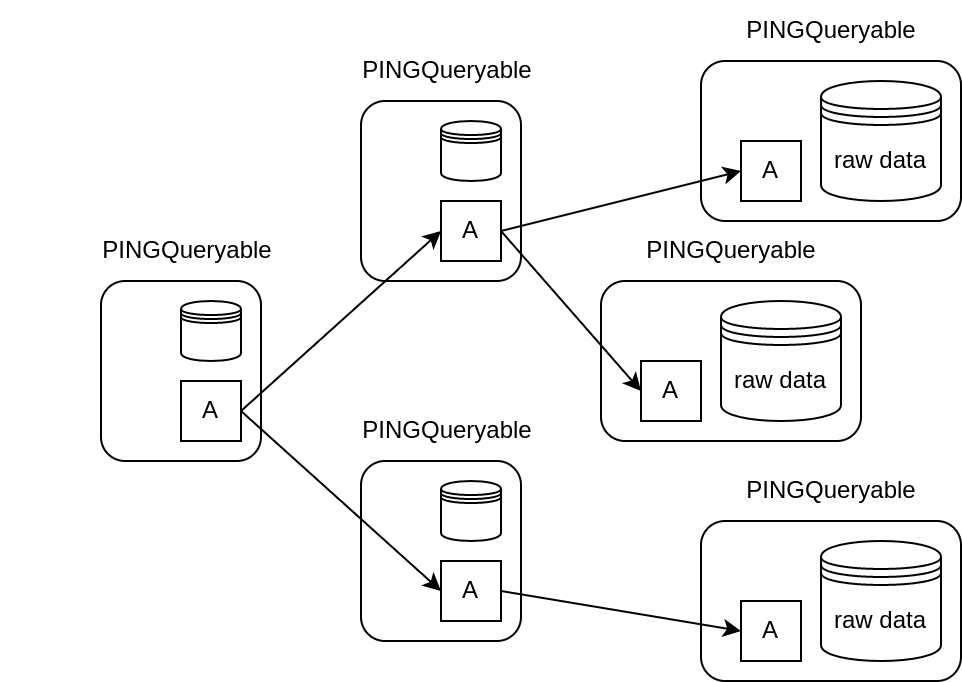
\includegraphics[width=0.55\textwidth]{example.drawio.png}
  \\\emph{Source}: \cite[]{mcsherry_privacy_2009}
  \caption{An example query structure linked via \texttt{PINQAgent}}\label{fig:example}
\end{wrapfigure}

Figure \ref{fig:example} shows an example structure of \texttt{PINQueryable} instances interlinked via their \texttt{PINQAgent}s (boxes with \enquote{A}) as might be produced with a moderately complex query.
This structure and the recursive \enquote{cost} calculation and authorization that it facilitates are an important feature of \gls[]{pinq}, because it informs the providers of the original data about the privacy implications of the queries that users run against them, as well as empowering them to accept or deny specific queries.
\parencite[]{mcsherry_privacy_2009}

Since \texttt{PINQAgent} is an extensible interface, data providers could implement their own custom logic for accepting and denying queries.
A simple implementation of the interface may be instantiated with a certain budget.
It would deny queries whose $\epsilon$ exceeds the budget and subtract the epsilon values of queries that it permits from the budget until it is exhausted. 
\parencite[]{mcsherry_privacy_2009}

Furthermore, they can offer different \texttt{PINQueryable} instances for different roles of users.
For example, if a data provider facilitates both access to internal and external analysts, they may offer the internal ones a \texttt{PINQueryable} instance with an \texttt{PINQAgent} that accepts all queries but logs them to some persistence, while for the external analysts a budget is enforced.
This flexibility and extensibility is another advantage of \gls[]{pinq}.
\parencite[]{mcsherry_privacy_2009}

\section{Conclusion}

The author shows a practical application of differential privacy to data analysis by designing and implementing a concise framework for a common, high-level programming language.
The goal of providing a generic foundation for privacy-preserving data analysis instead of complicated ad-hoc solutions to specific problems is commendable.
As is the focus on making privacy easy to implement for non-experts while empowering data providers.
Differential privacy and frameworks that make it easy to implement could, for example, play an important role in providing access to sensitive data for research purposes.

The electronic patient's record which is currently heavily debated in Germany is among other things also supposed to provide health data for research purposes.
To maintain the data owners' privacy, the data is supposed to be pseudonymised, which has drawbacks for the data analysis and might not prevent data leaks. \parencite[]{tagesschaude_gesundheitswesen_nodate}
Differential privacy could be a useful alternative here, to provide access to raw data with manageable privacy implications.

% BACKMATTER

\clearpage

% use roman numerals to number backmatter pages
\pagenumbering{Roman}

% use plain headers for backmatter pages
\pagestyle{plain.scrheadings}

% start numbering backmatter pages from 1
\setcounter{page}{\value{frontpagecount}}

% \pagestyle{empty}

% {
%   \centering\Huge\mbox{}
%   \vfill{}
%   Appendix\\
%   \vfill{}
% }

% \clearpage

\pagestyle{plain.scrheadings}

\appendix

% insert appendix sections here

\clearpage

% print bibliography in sloppypar environment for better URL placement
\begin{sloppypar}
  \printbibliography[
    heading=bibintoc % include bibliography in table of contents
  ]{}
\end{sloppypar}

\clearpage

\end{document}